\section{Results}
\label{sec:results}

\subsection{Cosine Similarity Across Layers (\gpttwo)}
\label{sec:cosine}

\Tabref{tab:cosine_gpt2} presents cosine similarity between clean and ciphered hidden states across layers in \gpttwo for all shuffle rates, alongside the random baseline and the permutation-adjusted condition.

\begin{table}[t]
    \centering
    \caption{Cosine similarity between clean and ciphered residual stream activations in \gpttwo across layers and shuffle rates. ``Adjusted'' applies the permutation-adjustment matrix $\permmat$ to ciphered states before comparison (full shuffle only). The random baseline uses non-bijective token replacement. Higher similarity at later layers is largely explained by architectural convergence (\cf \tabref{tab:intertext}).}
    \label{tab:cosine_gpt2}
    \begin{tabular}{@{}llccc@{}}
        \toprule
        Condition & $\shufflerate$ & Embedding & Layer 6 & Layer 12 \\
        \midrule
        Raw (clean vs.\ cipher) & 0.3 & 0.927 & 0.849 & 0.942 \\
        Raw (clean vs.\ cipher) & 0.5 & 0.873 & 0.756 & 0.912 \\
        Raw (clean vs.\ cipher) & 0.7 & 0.822 & 0.687 & 0.896 \\
        Raw (clean vs.\ cipher) & 1.0 & 0.743 & 0.579 & 0.873 \\
        \midrule
        Adjusted & 1.0 & 0.256 & 0.068 & 0.417 \\
        \midrule
        Random & --- & 0.637 & 0.526 & 0.858 \\
        \bottomrule
    \end{tabular}
\end{table}

Two patterns stand out. First, raw cosine similarity \emph{increases} from the middle layers to the final layer across all shuffle rates---at first glance suggesting recovery. Second, the random baseline also reaches 0.858 at the final layer, nearly matching the full-shuffle cipher (0.873). The permutation-adjusted similarity is dramatically \emph{lower} than raw similarity at every layer, reaching only 0.068 at layer 6. This directly refutes the hypothesis that the residual stream is ``normal modulo the shuffle''---undoing the cipher in embedding space introduces noise rather than recovering the clean representation.

\Figref{fig:cosine_layers} shows the full layer-by-layer trajectory.

\begin{figure}[t]
    \centering
    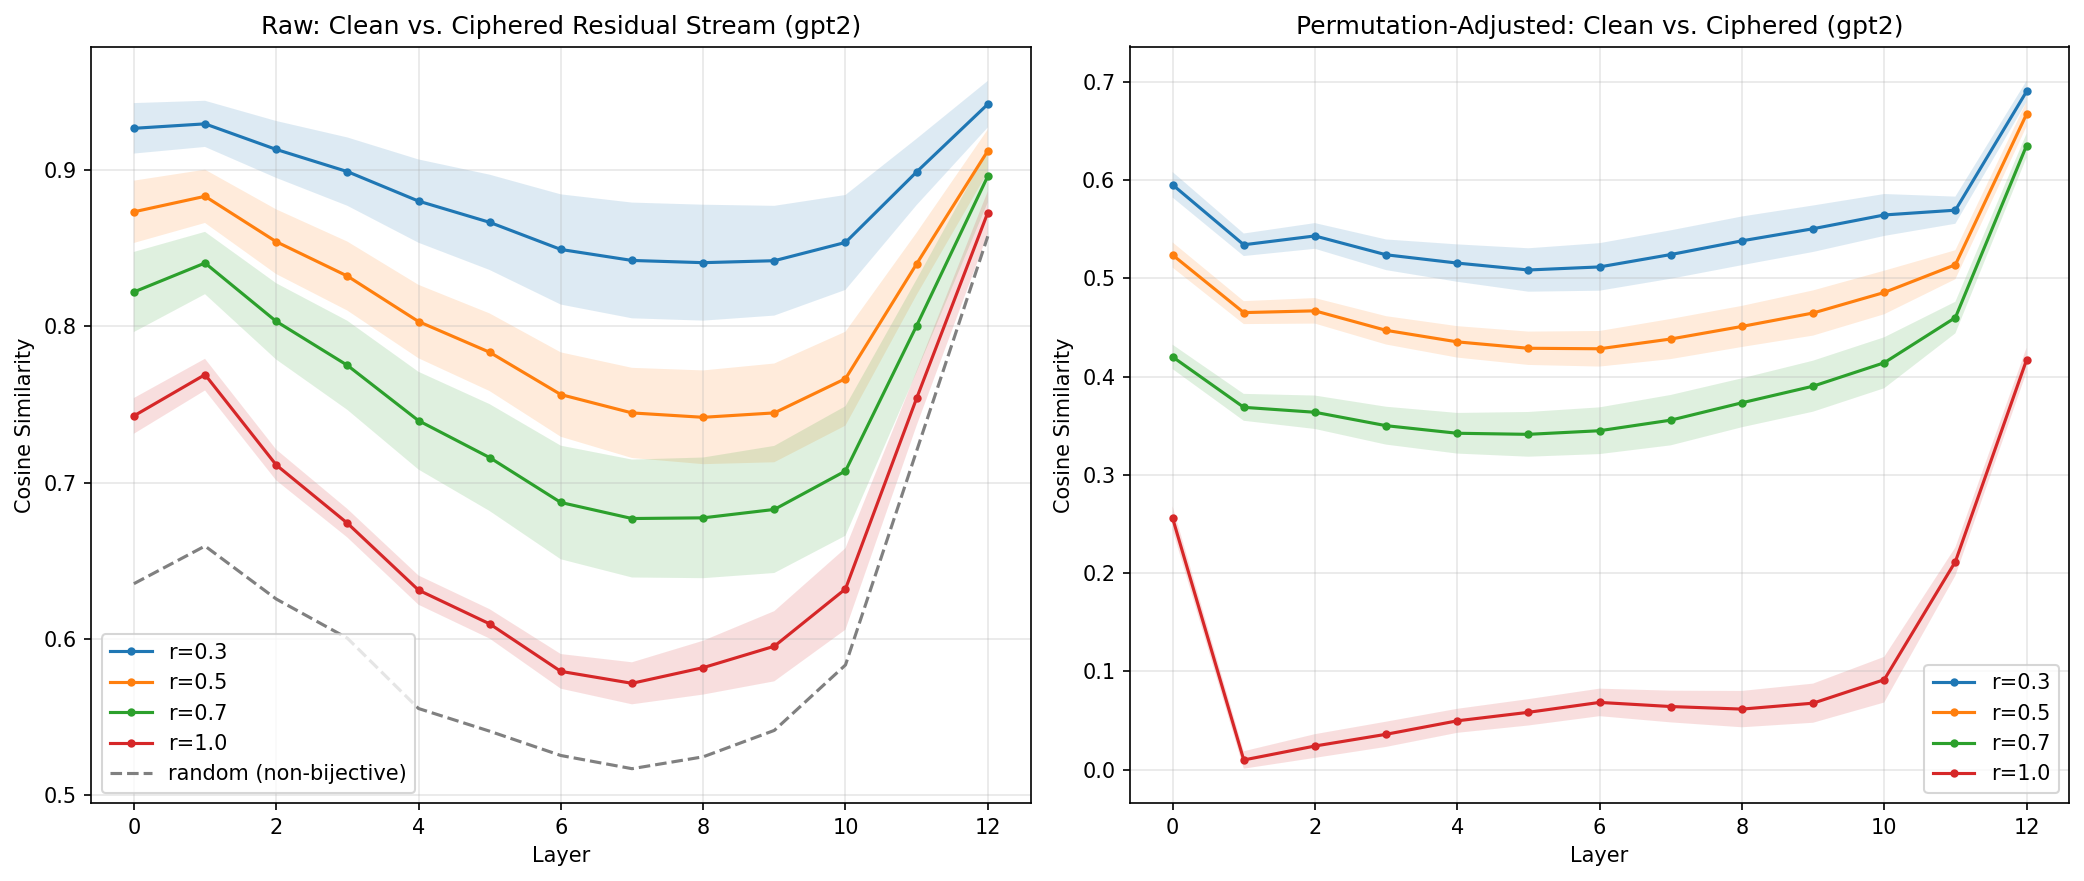
\includegraphics[width=0.95\linewidth]{figures/cosine_similarity_layers.png}
    \caption{Cosine similarity between clean and ciphered residual stream activations across all 12 layers of \gpttwo for shuffle rates $\shufflerate \in \{0.3, 0.5, 0.7, 1.0\}$, alongside the random baseline and permutation-adjusted condition. All conditions converge toward high similarity at later layers, but the random baseline tracks closely, indicating this is an architectural artifact. The adjusted condition remains low throughout.}
    \label{fig:cosine_layers}
\end{figure}

\subsection{Architectural Convergence Control}
\label{sec:convergence}

\Tabref{tab:intertext} reveals the source of the high later-layer similarity: \layernorm drives all representations toward similar directions regardless of input content.

\begin{table}[t]
    \centering
    \caption{Cosine similarity between position-averaged hidden states of \emph{different clean texts} in \gpttwo. The consistently high similarity ($>0.96$) at all layers demonstrates that \layernorm forces representations into a narrow cone, explaining why ciphered and random inputs also achieve high similarity at later layers.}
    \label{tab:intertext}
    \begin{tabular}{@{}lc@{}}
        \toprule
        Layer & Inter-text Similarity \\
        \midrule
        0 & 0.963 \\
        3 & 0.996 \\
        6 & 0.994 \\
        9 & 0.986 \\
        12 & 0.963 \\
        \bottomrule
    \end{tabular}
\end{table}

Different clean texts---with entirely different content---already show $>$0.96 cosine similarity at every layer. This means the high clean-vs-cipher similarity (0.873 at layer 12 for full shuffle) is \emph{not} evidence of cipher decoding. It is a property of the architecture itself.

\subsection{Cross-Model Validation (\pythia)}
\label{sec:pythia}

To verify that our findings are not specific to \gpttwo, we repeat the analysis on \pythia, which uses a different normalization scheme and exhibits weaker architectural convergence.

\begin{table}[t]
    \centering
    \caption{Residual stream similarity in \pythia across shuffle rates. Unlike \gpttwo, \pythia shows clearer separation between conditions. CKA provides a rotation-invariant comparison. The cipher sits above random but below clean, with similarity \emph{decreasing} from embedding to final layer at low shuffle rates.}
    \label{tab:pythia}
    \begin{tabular}{@{}lccc@{}}
        \toprule
        Condition ($\shufflerate$) & Embedding & Final Layer & CKA (Final) \\
        \midrule
        Raw (0.3) & 0.766 & 0.688 & 0.603 \\
        Raw (0.5) & 0.581 & 0.565 & 0.509 \\
        Raw (1.0) & 0.146 & 0.391 & 0.300 \\
        \midrule
        Random & --- & 0.295 & --- \\
        \bottomrule
    \end{tabular}
\end{table}

\Pythia tells a more nuanced story (\tabref{tab:pythia}; \figref{fig:pythia}). The cipher produces representations 30\% above random (0.391 vs.\ 0.295 at the final layer for full shuffle) but 30\% below clean. Importantly, similarity \emph{decreases} from embedding to final layer at low shuffle rates (0.766 $\to$ 0.688 for $\shufflerate = 0.3$), contrary to a recovery hypothesis. The model extracts some distributional structure from ciphered text---co-occurrence patterns survive the bijection---but does not decode the cipher.

\begin{figure}[t]
    \centering
    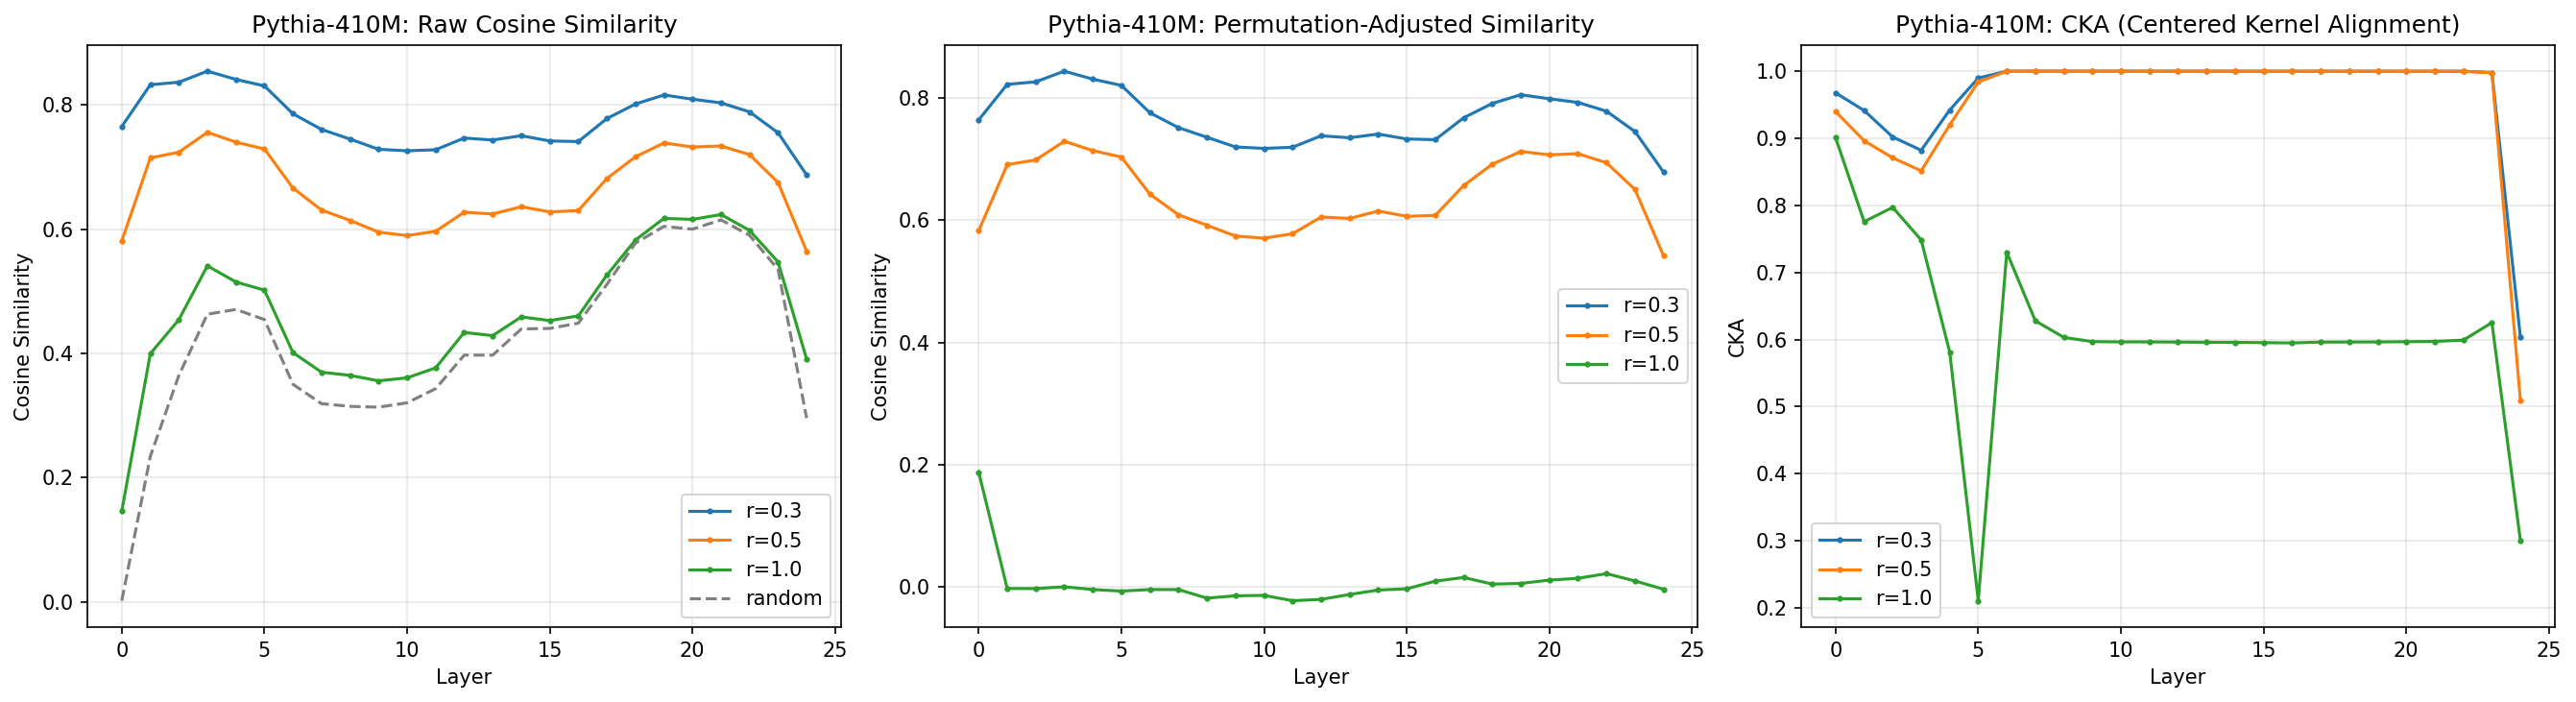
\includegraphics[width=0.95\linewidth]{figures/pythia_analysis.png}
    \caption{\Pythia residual stream analysis showing raw cosine similarity, permutation-adjusted similarity, and CKA across layers. The weaker architectural convergence in \pythia reveals clearer separation between cipher and random conditions, but no evidence of recovery toward clean representations.}
    \label{fig:pythia}
\end{figure}

\subsection{Logit Lens Analysis}
\label{sec:logitlens}

The logit lens provides the most direct test of whether the model decodes the cipher: does it predict the correct next token under the cipher mapping?

\begin{table}[t]
    \centering
    \caption{Logit lens results: mean rank of the target next token at the final layer of \gpttwo (out of 50{,}257 tokens). ``Cipher-correct'' is the token that \emph{should} follow under the cipher mapping; ``Original'' is the un-ciphered correct token. Both have essentially random ranks under cipher, confirming no decoding occurs. Best (lowest) rank in \textbf{bold}.}
    \label{tab:logitlens}
    \begin{tabular}{@{}llc@{}}
        \toprule
        Condition & Target Token & Mean Rank \\
        \midrule
        Clean & Correct next token & \textbf{166} \\
        Cipher ($\shufflerate = 0.3$) & Cipher-correct & 5{,}909 \\
        Cipher ($\shufflerate = 0.5$) & Cipher-correct & 7{,}787 \\
        Cipher ($\shufflerate = 1.0$) & Cipher-correct & 11{,}542 \\
        Cipher ($\shufflerate = 1.0$) & Original token & 11{,}607 \\
        \bottomrule
    \end{tabular}
\end{table}

\Tabref{tab:logitlens} shows that the model emphatically does not decode the cipher. Under clean text, the correct next token has a mean rank of 166---reasonable for a language model. Under the full cipher, the cipher-consistent next token has rank 11{,}542, and the original (un-ciphered) next token has rank 11{,}607. Both are essentially random out of 50{,}257 tokens. The model predicts neither the ciphered nor the original token---it is simply lost. \Figref{fig:logitlens} shows the rank trajectory across layers.

\begin{figure}[t]
    \centering
    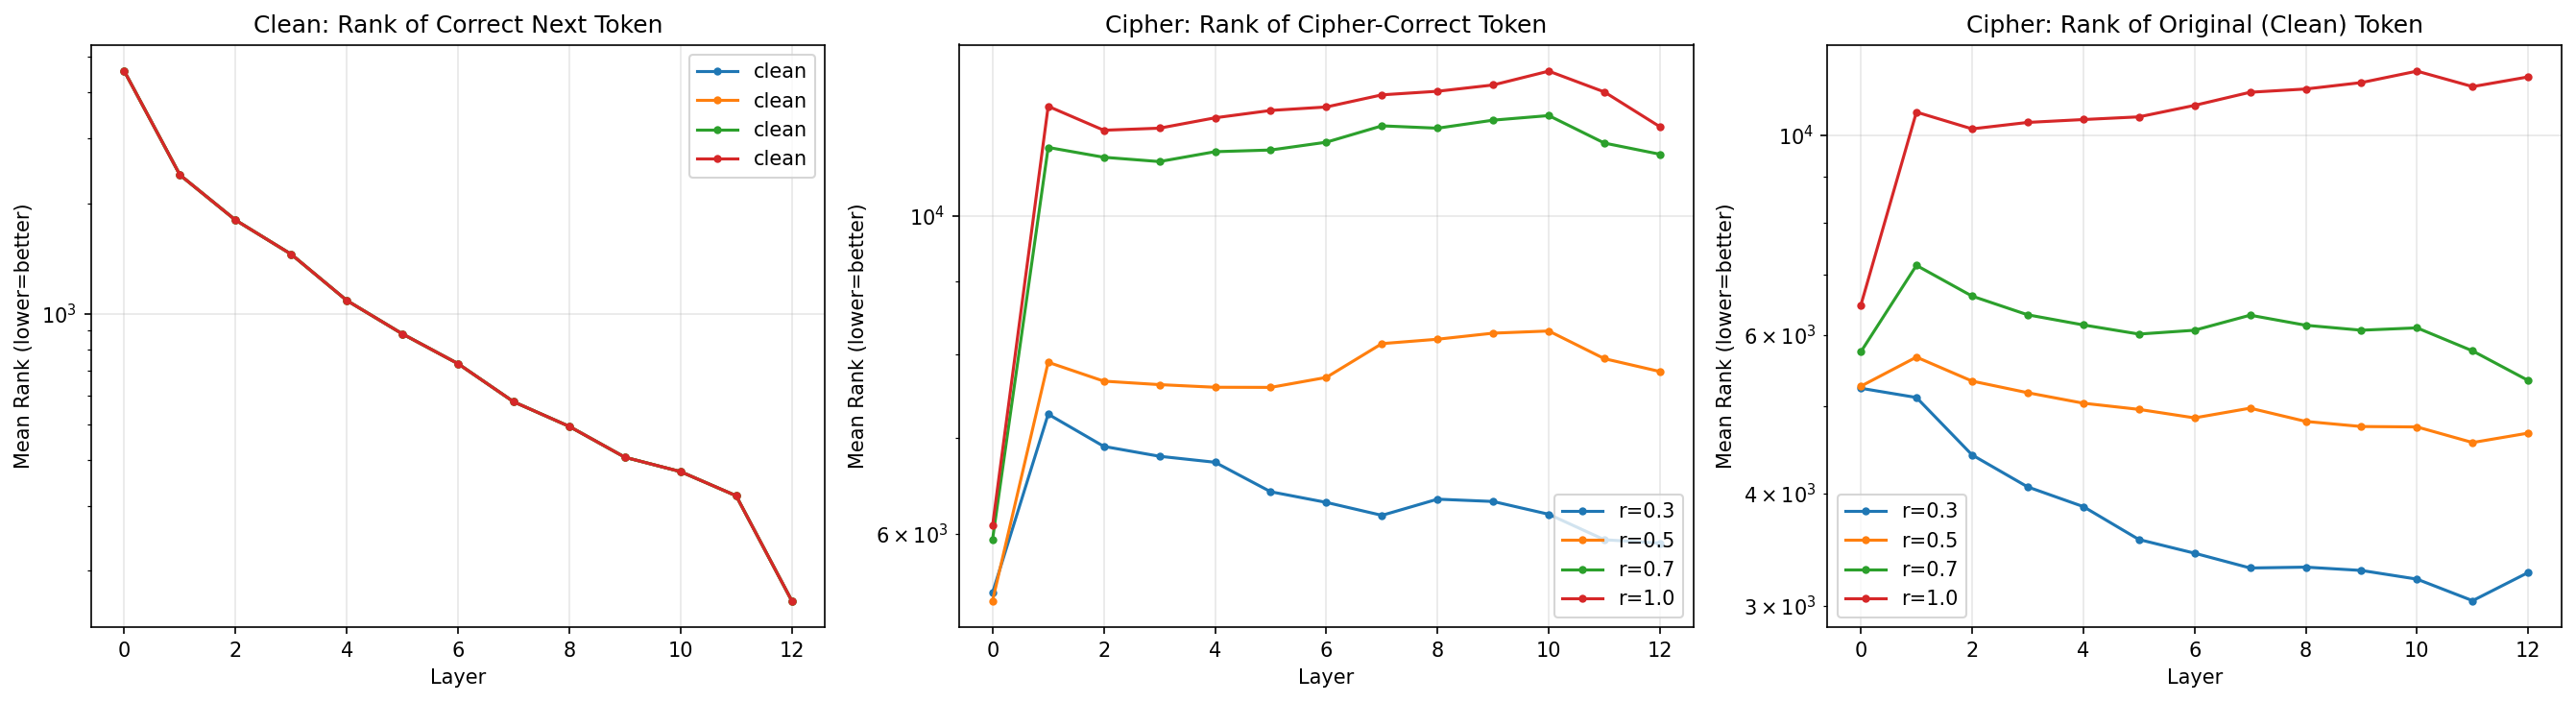
\includegraphics[width=0.95\linewidth]{figures/logit_lens_ranks.png}
    \caption{Logit lens token rank across layers of \gpttwo for clean and ciphered conditions. Under clean text, the correct next token's rank steadily improves (decreases) through the layers. Under cipher, the rank remains flat and high at all layers, confirming no progressive cipher decoding occurs.}
    \label{fig:logitlens}
\end{figure}

\subsection{Attention Pattern Analysis}
\label{sec:attention}

\begin{table}[t]
    \centering
    \caption{Attention entropy (nats) averaged across heads and positions in \gpttwo. Cipher text produces slightly higher entropy at later layers, indicating mild uncertainty in attention allocation, but the difference is small.}
    \label{tab:attention}
    \begin{tabular}{@{}lcc@{}}
        \toprule
        Layer & Clean & Cipher ($\shufflerate = 1.0$) \\
        \midrule
        0  & 1.038 & 1.054 \\
        3  & 0.877 & 0.847 \\
        6  & 0.704 & 0.669 \\
        9  & 0.478 & 0.529 \\
        11 & 0.710 & 0.811 \\
        \bottomrule
    \end{tabular}
\end{table}

Attention patterns are only mildly affected by the cipher (\tabref{tab:attention}). At layer 11, cipher text produces modestly higher entropy (0.811 vs.\ 0.710 nats), indicating the model is slightly less certain about which positions to attend to. However, the overall attention structure---dominated by positional priors and local context---remains largely intact. This suggests the attention mechanism operates on positional and structural cues that survive the token permutation.

\subsection{Statistical Significance}
\label{sec:stats}

\begin{table}[t]
    \centering
    \caption{Paired $t$-tests comparing raw cipher similarity to random baseline at layers 6--12 of \gpttwo. The cipher consistently produces higher similarity than random ($p < 0.001$), but the effect is small relative to the architectural convergence floor.}
    \label{tab:stats}
    \begin{tabular}{@{}lcccc@{}}
        \toprule
        $\shufflerate$ & Raw Mean & Random Mean & $t$ & $p$ \\
        \midrule
        0.3 & 0.926 & 0.800 & 7.41 & 0.0003 \\
        0.5 & 0.898 & 0.800 & 7.02 & 0.0004 \\
        0.7 & 0.876 & 0.799 & 6.92 & 0.0004 \\
        1.0 & 0.847 & 0.800 & 7.48 & 0.0003 \\
        \bottomrule
    \end{tabular}
\end{table}

The cipher consistently produces significantly higher similarity than random replacement across all shuffle rates ($p < 0.001$; \tabref{tab:stats}). This confirms that the bijective structure provides \emph{some} signal beyond random noise---likely because frequency-matched permutations preserve distributional statistics that the model partially extracts. However, this statistical significance should be interpreted against the architectural convergence baseline: the gap between cipher (0.847) and random (0.800) at $\shufflerate = 1.0$ is much smaller than the gap between either condition and the inter-text clean baseline ($>0.96$).
